\documentclass{article}
\usepackage{amsmath}
\usepackage{amsfonts}
\usepackage{bm}
\usepackage{graphicx}
\usepackage{float}
\usepackage{subfigure}
\usepackage{enumitem}
\usepackage{ctex}

\renewcommand{\figurename}{Figure}
\renewcommand{\thesubfigure}{}

\begin{document}
\begin{titlepage}
\vspace*{\fill}
\begin{center}
\huge Wireless Communication Systems \\HW3\\ 109064509 楊暐之
\end{center}
\vspace{\fill}
\end{titlepage}

\begin{flushleft}
For simplicity, I set $T=1$ for all cases in my simulation.\\[0.5cm]
\begin{enumerate}
%% Filtered Gaussian Noise Method
{\Large \item  \bf Filtered Gaussian Noise Method : }\\
I use first-order low-pass digital filter to generate the channel output as following
\begin{equation}
\begin{pmatrix}g_{I,k+1}\\g_{Q,k+1}\end{pmatrix}=\zeta\begin{pmatrix}g_{I,k}\\g_{Q,k}\end{pmatrix}+(1-\zeta)\begin{pmatrix}w_{1,k}\\w_{2,k}\end{pmatrix} 
\end{equation}
$\begin{aligned}
\mathrm {where}\ &g_{I,k},g_{Q,k}\ {\rm are\ in-phase\ and\ quadrature\ component\ at\ time\ }kT\\
&w_{1,k} , w_{2,k}\overset{iid}\sim\mathcal N(0,\sigma^2)\\
&\zeta=2-\cos\left(\frac{\pi f_mT}{2}\right)-\sqrt{\left(2-\cos\left(\frac{\pi f_mT}{2}\right)\right)^2-1}\\
&\sigma^2=\left(\frac{1+\zeta}{1-\zeta}\right)\frac{\Omega_p}{2},\ \frac{\Omega_p}{2}\ {\rm is\ the\ PSD\ of\ input\ noise\ source}
\end{aligned}$\\[0.2cm]
and I use the equation at the lecture note CH2-p93 to simulate the autocorrelation $\phi_{g_Ig_I}$
\begin{equation}
\phi_{g_Ig_I}(n)=\phi_{g_Qg_Q}(n)=\frac{1-\zeta}{1+\zeta}\sigma^2\zeta^{|n|}\notag
\end{equation}
Furthermore, because I generate the output  by (1) with initial value $g_{I,0},g_{Q,0}$(here I set 0 for both), the value of envelope level around 0 is significantly affected by the initial value, so I use the last 300 points of $g$ instead

\newpage
%%envelope
\begin{figure}[H]
\centering
\subfigure[(a)]{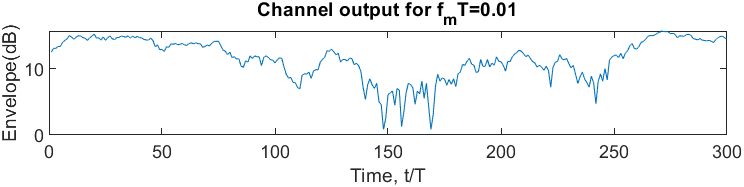
\includegraphics[width=0.9\textwidth]{1_env_1}}
\subfigure[(b)]{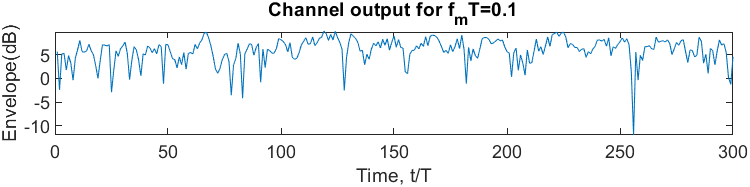
\includegraphics[width=0.9\textwidth]{1_env_2}}
\subfigure[(c)]{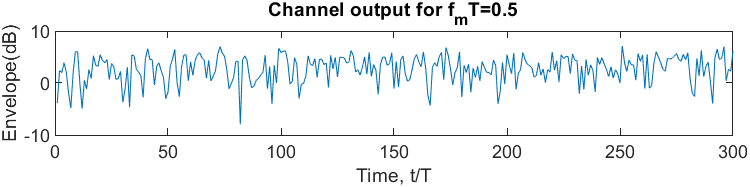
\includegraphics[width=0.9\textwidth]{1_env_3}}
\caption{Envelope level(dB) of channel output (a)$f_mT=0.01$ \\(b)$f_mT=0.1$ (c)$f_mT=0.5$}
\end{figure}
$f_mT \uparrow\ \Rightarrow\ \zeta \downarrow\ \Rightarrow\ (1-\zeta)\uparrow $\\
Thus, as $f_mT$ become large, the noise affects ouput more seriously

\newpage
%%Autocorrelation with normalization
\begin{figure}[H]
\centering
\subfigure[(a)]{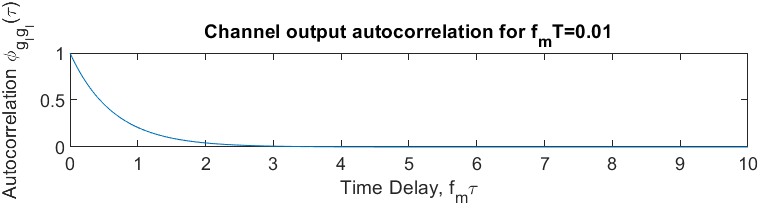
\includegraphics[width=0.9\textwidth]{1_Rn_1}}
\subfigure[(b)]{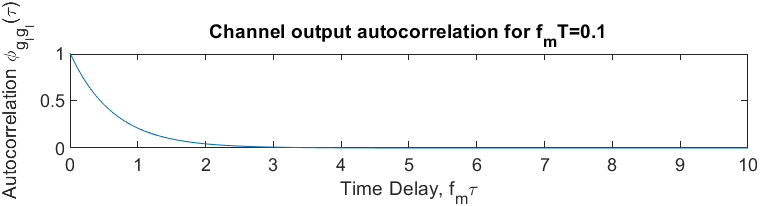
\includegraphics[width=0.9\textwidth]{1_Rn_2}}
\subfigure[(c)]{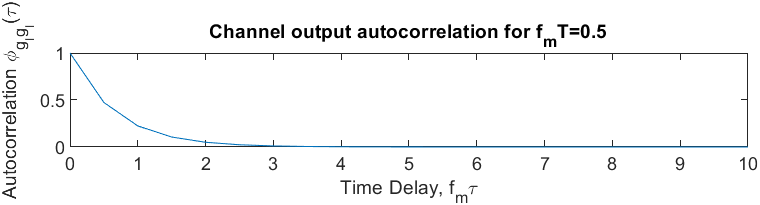
\includegraphics[width=0.9\textwidth]{1_Rn_3}}
\caption{Autocorrelation with normalization of in-phase component of channel output (a)$f_mT=0.01$ (b)$f_mT=0.1$ (c)$f_mT=0.5$}
\end{figure}
Since the channel output is $g(t)=g_I(t)+jg_Q(t)$, the autocorrelation of channel output is given as
\begin{equation}
\phi_{gg}(\tau)=2\phi_{g_Ig_I}(\tau)=2\phi_{g_Qg_Q}(\tau)\notag
\end{equation}
Thus, I present the autocorrelation $\phi_{g_Ig_I}(\tau)$ instead.\\
And due to normalization, Figure 2-(a), 2-(b), 2-(c) are look like the same. I will show non-normalized results later

\newpage
%%Autocorrelation without normalization
\begin{figure}[H]
\centering
\subfigure[(a)]{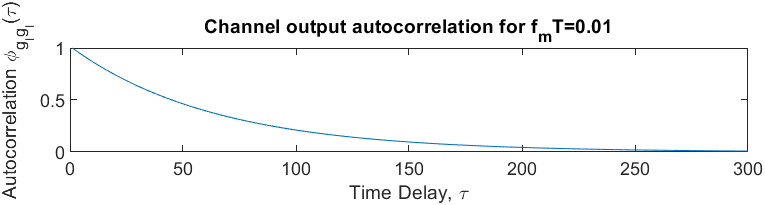
\includegraphics[width=0.9\textwidth]{1_R_1}}
\subfigure[(b)]{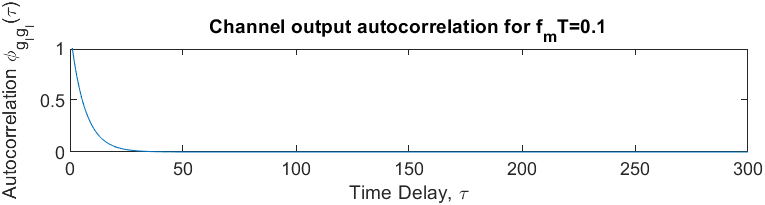
\includegraphics[width=0.9\textwidth]{1_R_2}}
\subfigure[(c)]{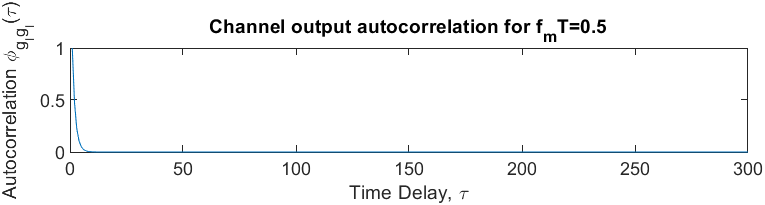
\includegraphics[width=0.9\textwidth]{1_R_3}}
\caption{Autocorrelation without normalizationof in-phase component of channel output (a)$f_mT=0.01$ (b)$f_mT=0.1$ (c)$f_mT=0.5$}
\end{figure}
Without normalization, it is easy to see that as $f_m$ become large,  $\phi_{g_Ig_I}(\tau)$ decays more rapidly

\newpage
%% Sum of Sinusoids Method
{\Large \item  \bf Sum of Sinusoids Method : }\\
I generate the channel output as following\\
$\begin{aligned}
g(t)=&g_I(t)+jg_Q(t)\\
=&2\sqrt{2}\left\{\left[\sum\limits_{n=1}^M \cos(\beta_n)\cos(2\pi f_nt) \right]+j\left[\sum\limits_{n=1}^M \sin(\beta_n)\cos(2\pi f_nt) \right] \right\}
\end{aligned}$
where I ignored the term of $\cos(\alpha)\cos(2\pi f_mt)$ of $g_I(t)$ and the term of $\sin(\alpha)\cos(2\pi f_mt)$ of $g_Q(t)$ is equal to 0 as choose $\alpha=0$\\
Note that $\beta_n=\frac{\pi n}{M},\ f_n=f_m\cos(\theta_n)$, where $ \theta_n=\frac{2\pi n}{N}$\\
And I simulate the autocorrelation by using the MATLAB function autocorr

\newpage
%% envelope M=8
\begin{figure}[H]
\centering
\subfigure[(a)]{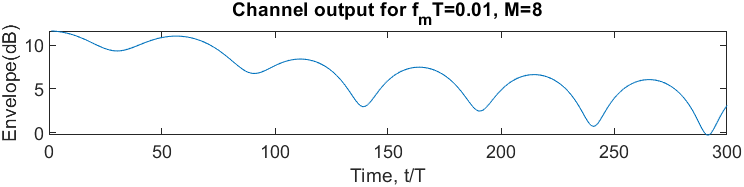
\includegraphics[width=0.9\textwidth]{2_8_env_1}}
\subfigure[(b)]{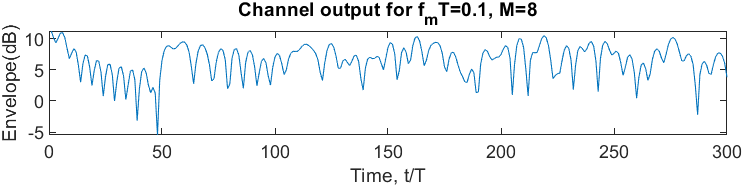
\includegraphics[width=0.9\textwidth]{2_8_env_2}}
\subfigure[(c)]{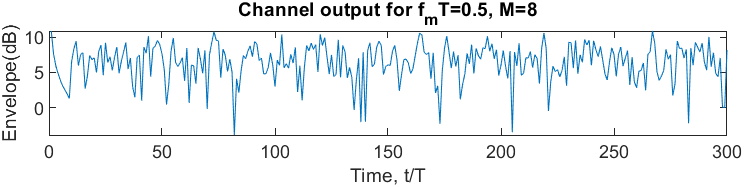
\includegraphics[width=0.9\textwidth]{2_8_env_3}}
\caption{Envelope level(dB) of channel output for $M=8$ (a)$f_mT=0.01$ (b)$f_mT=0.1$ (c)$f_mT=0.5$}
\end{figure}
Since the initial phase(the phase at $t=0$) is 0 for all sinusoid components of $g_I,g_Q$, it occurs constructive interferences around $t=0$.Thus, the envelope level get relatively large value around $t=0$\\
Otherwise, as $f_m$ become larger, the output of channel is more noise-like


\newpage
%% envelope M=16
\begin{figure}[H]
\centering
\subfigure[(a)]{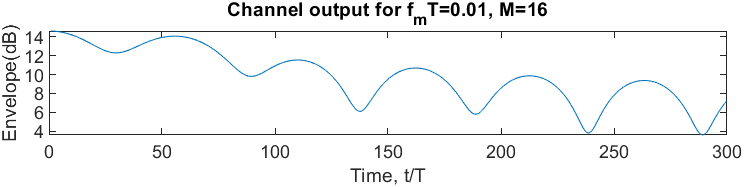
\includegraphics[width=0.9\textwidth]{2_16_env_1}}
\subfigure[(b)]{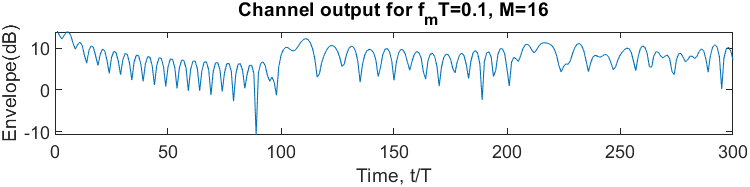
\includegraphics[width=0.9\textwidth]{2_16_env_2}}
\subfigure[(c)]{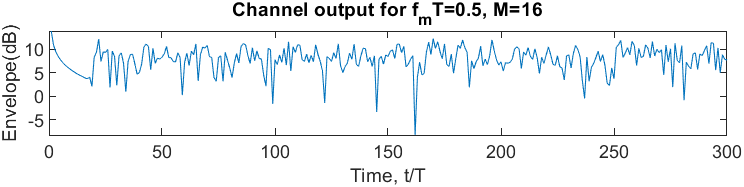
\includegraphics[width=0.9\textwidth]{2_16_env_3}}
\caption{Envelope level(dB) of channel output for $M=16$ (a)$f_mT=0.01$ (b)$f_mT=0.1$ (c)$f_mT=0.5$}
\end{figure}
Compare the case of $M=8$ with $M=16$,we can observe that the duration of constructive interference around $t=0$ of $M=16$ is longer than $M=8$

\newpage
%% autocorrelation M=8
\begin{figure}[H]
\centering
\subfigure[(a)]{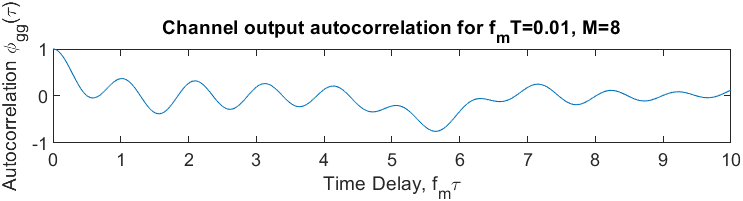
\includegraphics[width=0.9\textwidth]{2_8_Rn_1}}
\subfigure[(b)]{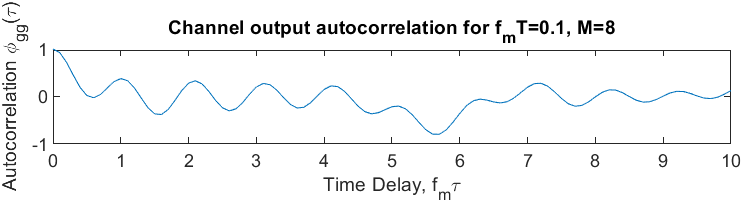
\includegraphics[width=0.9\textwidth]{2_8_Rn_2}}
\subfigure[(c)]{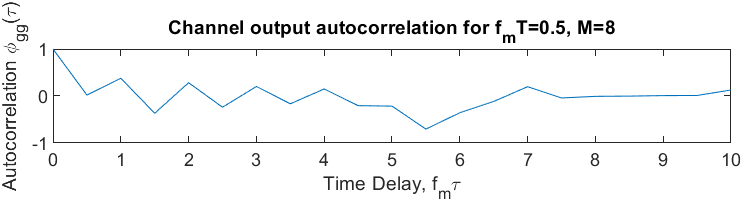
\includegraphics[width=0.9\textwidth]{2_8_Rn_3}}
\caption{Autocorrelation with normalization of channel output for $M=8$ (a)$f_mT=0.01$ (b)$f_mT=0.1$ (c)$f_mT=0.5$}
\end{figure}
We can observe that the value of autocorrelation is much inaccurate after $f_m\tau=6$ no matter what the value of $f_mT$ is 


\newpage
%% autocorrelation M=16
\begin{figure}[H]
\centering
\subfigure[(a)]{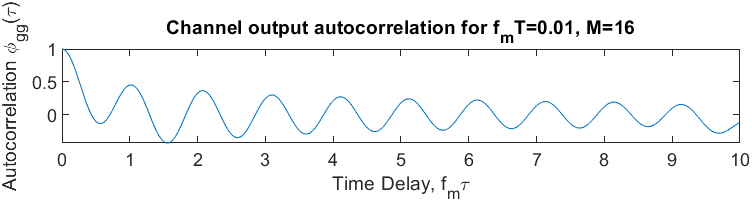
\includegraphics[width=0.9\textwidth]{2_16_Rn_1}}
\subfigure[(b)]{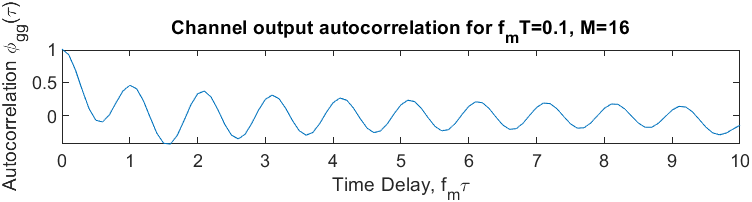
\includegraphics[width=0.9\textwidth]{2_16_Rn_2}}
\subfigure[(c)]{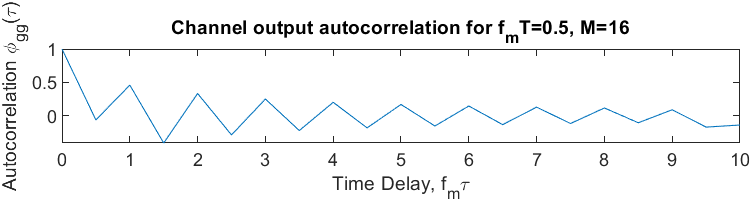
\includegraphics[width=0.9\textwidth]{2_16_Rn_3}}
\caption{Autocorrelation with normalization of channel output for $M=16$  (a)$f_mT=0.01$ (b)$f_mT=0.1$ (c)$f_mT=0.5$}
\end{figure}
As we increase $M$ to 16, the value of autocorrelation is more accurate

\newpage
%% Discussion 
{\Large \item  \bf Discussion : }\\
\ \ Compare the envelope level and autocorrelation generated by Filtered Gaussian Noise Method with Sum of Sinusoids Method, we can see that the envelope level generated by Filtered Gaussian Noise Method is more noise-like, and maintain the randomness. For Sum of Sinusoids Method, even though we can choose different start time to get the property that is similar to ramdomness, it is still a deterministic periodic signal indeed.
However, as $M$ is sufficient large, the value of autocorrelation generated by  Sum of Sinusoids Method is much more like the real value of autocorrelation than Filtered Gaussian Noise Method.

\end{enumerate}
\end{flushleft}



\end{document}